%%%%%%%%%%%%%%%%%%%%%%%%%%%%%%%%%%%%%%%%%%%%%%%%%%%%%%%%%%%%%%%%%%
%	@file Vorlage.tex
%	@author David Pfahler (1126287) <e1126287@student.tuwien.ac.at>
% 
% If something doesn't work feel free to write me a mail
%%%%%%%%%%%%%%%%%%%%%%%%%%%%%%%%%%%%%%%%%%%%%%%%%%%%%%%%%%%%%%%%%%


\documentclass[11pt]{scrartcl}
\usepackage{secVorlage}

\secTitle{HAx/Projektx - Title}
\secDate{\today}
\secAuthors{
\begin{table}[htbp]
		\centering
			\begin{tabular}{>{\itshape}p{4cm} >{\itshape}c >{\itshape}p{4cm}}
				Student1  & 1234567 & \href{mailto:e1234567@student.tuwien.ac.at}{e1234567@student.tuwien.ac.at}\\
				Student2  & 1234567 & \\
				Student3  & 1234567 & \\
				Student4  & 1234567 & \\
			\end{tabular}
	\end{table}	
}

\begin{document}
	
\createSecTitle


\section{Introduction}
Congratulations! Your paper has been accepted for journal publication. Please follow the steps outlined below when submitting your final draft to the SERSC Press. These guidelines include complete descriptions of the fonts, spacing, and related information for producing your proceedings manuscripts. Please follow them and if you have any questions, direct them to the production editor in charge of your journal at the SERSC, sersc@sersc.org.

\section{Formatting your paper}
All printed material, including text, illustrations, and charts, must be kept within the parameters of the 8 15/16-inch (53.75 picas) column length and 5 15/16-inch (36 picas) column width. Please do not write or print outside of the column parameters. Margins are 1 5/16 of an inch on the sides (8 picas), 7/8 of an inch on the top (5.5 picas), and 1 3/16 of an inch on the bottom (7 picas).

\section{Main title}
The main title (on the first page) should begin 1 3/16 inches (7 picas) from the top edge of the page, centered, and in Times New Roman 14-point, boldface type. Capitalize the first letter of nouns, pronouns, verbs, adjectives, and adverbs; do not capitalize articles, coordinate conjunctions, or prepositions (unless the title begins with such a word). Please initially capitalize only the first word in other titles, including section titles and first, second, and third-order headings (for example, “Titles and headings” — as in these guidelines). Leave two blank lines after the title.

\section{Second and following pages}
The second and following pages should begin 1.0 inch (2.54 cm) from the top edge. On all pages, the bottom margin should be 1-3/16 inches (2.86 cm) from the bottom edge of the page for 8.5 x 11-inch paper; for A4 paper, approximately 1-5/8 inches (4.13 cm) from the bottom edge of the page.

\section{Type-style and fonts}
Wherever Times New Roman is specified, Times Roman, or Times may be used. If neither is available on your word processor, please use the font closest in appearance to Times New Roman that you have access to. Please avoid using bit-mapped fonts if possible. True-Type 1 fonts are preferred.

\begin{table}[tbh]
	\caption{Sample Table}
	\centering
		\begin{tabular}{|l|l|l|}
				\hline
				test&test&test\\
				\hline
				test&test&test\\
				\hline
				test&test&test\\
				\hline
		\end{tabular}
	\label{tab:SampleTable}
\end{table}

\begin{figure}[tbh]
	\centering
		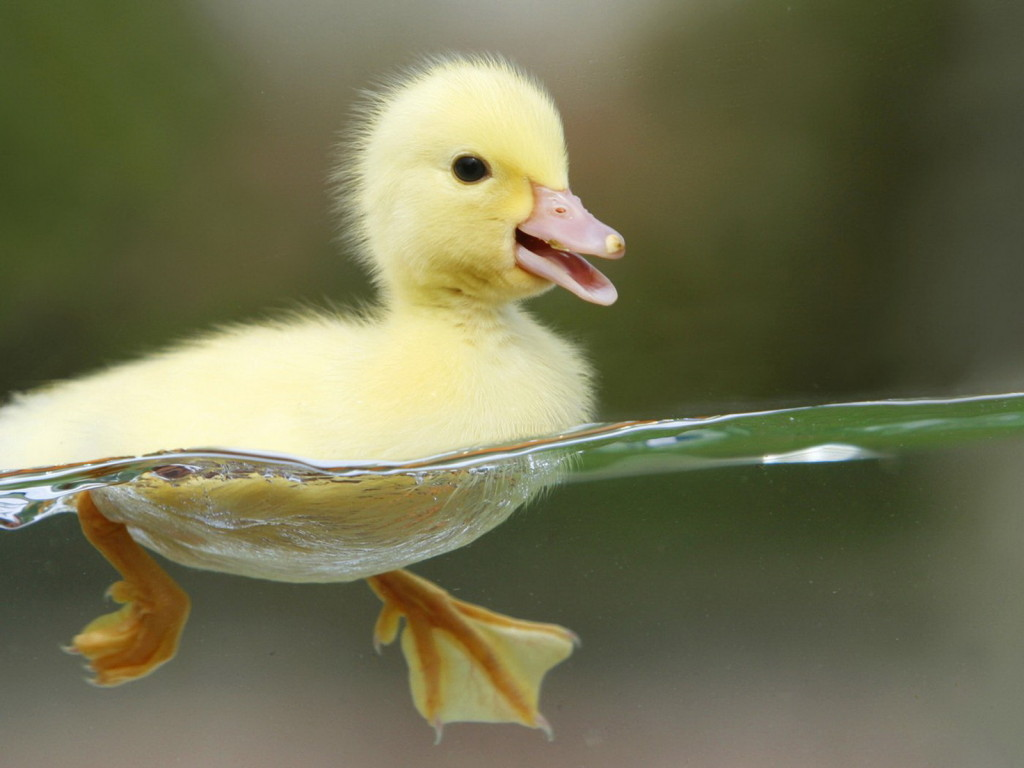
\includegraphics[width=0.50\textwidth]{Example.jpg}
	\caption{This is an example image}
	\label{fig:example}
\end{figure}

\section{Main text}
Type your main text in 11-point Times New Roman, single-spaced with 13-point interline spacing. Do not use double-spacing. All paragraphs should be indented 1 pica (approximately 1/6- or 0.17-inch or 0.422 cm). Be sure your text is fully justified—that is, flush left and flush right. Please do not place any additional blank lines between paragraphs. 
Figure and table captions should be 11-point Helvetica boldface (or a similar sans-serif font). Callouts should be 10-point Helvetica, non-boldface. Initially capitalize only the first word of each figure caption and table title. Figures and tables must be numbered separately. For example: \autoref{fig:example}, \autoref{tab:SampleTable}. Figure captions are to be below the figures. Table titles are to be centered above the tables.

\section{First-order headings}
For example, “1. Introduction”, should be Times New Roman 13-point boldface, initially capitalized, flush left, with one blank line before, and one blank line after. Use a period (“.”) after the heading number, not a colon.

\subsection{Second-order headings}
As in this heading, they should be Times New Roman 11-point boldface, initially capitalized, flush left, with one blank line before, and one after.

\subsubsection{Third-order headings} Are not necessary in articles up to 20 pages.

\section{Footnotes}
Use footnotes\footnote{This is a footnote} sparingly (or not at all!) and place them at the bottom of the column on the page on which they are referenced. Use Times New Roman 9-point type, single-spaced with 10-point interlining spacing. To help your readers, avoid using footnotes altogether and include necessary peripheral observations in the text (within parentheses, if you prefer, as in this sentence).

\section{Enumerations}
There were no restrications to enumerations.. so i used the standard \LaTeX -enums. If you dont want a too big spacing between the items use the commands: \texttt{$\backslash$begin\{myitem\}} and \texttt{$\backslash$begin\{myenum\}} which provide a smaller gap.

\begin{enumerate}
	\item Item 1
	\item Item 2
	\item Item 3
	\begin{enumerate}
		\item Item 3.1
		\item Item 3.2
		\item Item 3.3
	\end{enumerate}
\end{enumerate}

\begin{itemize}
	\item Item 1
	\item Item 2
	\item Item 3
	\begin{itemize}
		\item 3.1
		\item 3.2
	\end{itemize}
\end{itemize}

\section{ACKNOWLEDGEMENTS}

These should be brief and placed at the end of the text before the references.

\section{References}

\fontsize{9}{10pt}
\bibliographystyle{plain}
%I didn't test anything here! maybe a different bibliographystyle?

List and number all bibliographical references in 9-point Times New Roman, single-spaced with 10-point interlining spacing, at the end of your paper. When referenced in the text, enclose the citation number in square brackets, for example \cite{1}. Where appropriate, include the name(s) of editors of referenced books.

\bibliography{references}

\end{document}
